\section{Mainboard}

\begin{frame}
	\setbeamercovered{transparent}
	\frametitle{Mainboard}
	
	\begin{columns}
		\begin{column}{0.5\textwidth}
			\begin{itemize}
				\item Neue Hardware
				\item Neue oder überarbeitete Module:
				\begin{itemize}
					\item Bluetooth Kommunikation
					\item Display
					\item CAN Kommunikation
				\end{itemize}
			\end{itemize}
		\end{column}
	
		\begin{column}{0.5\textwidth}
			\begin{figure}
				\includegraphics[width=0.8\textwidth]{../images/tiva_tm4c1294xl_ek.jpg}
			\end{figure}
		\end{column}
	\end{columns}
\end{frame}

\begin{frame}
	\frametitle{Mainboard}
	\framesubtitle{Bluetooth Kommunikation}
	
	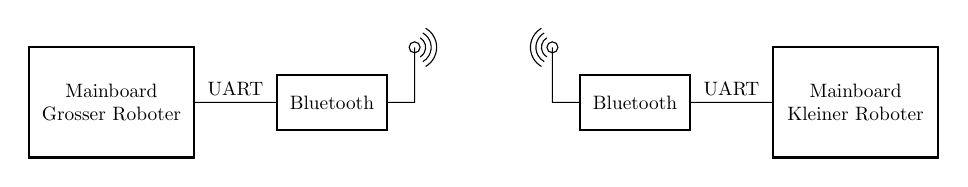
\begin{tikzpicture}[scale=0.7, transform shape]
		%grosser roboter 
		
		%mainboard
		\draw[thick] (0.5,0.5) coordinate (big mb) rectangle ++(3,2) node[pos=0.5, align=center]{Mainboard\\Grosser Roboter}; 
		\draw (big mb) ++ (3,1) coordinate (big mb uart);
		%btDongle
		\draw[thick] (5,1) coordinate (big bt) rectangle ++(2,1) node[pos=0.5]{Bluetooth};
		\draw (big bt) ++ (0,0.5) coordinate (big bt uart);
		\draw (big bt) ++ (2,0.5) coordinate (big bt bt);
		\draw (big bt bt) -- ++ (0.5,0) -- ++ (0,1) circle (0.1) coordinate (big bt antenna);
		\foreach \r in {.2,.3,.4}
		\draw (big bt antenna) ++ (60:\r) arc (60:-60:\r);
		
		%kleiner Roboter
		%btDongle
		\draw[thick] (10.5,1) coordinate (small bt) rectangle ++(2,1) node[pos=0.5]{Bluetooth};
		\draw (small bt) ++ (2,0.5) coordinate (small bt uart);
		\draw (small bt) ++ (0,0.5) coordinate (small bt bt);
		\draw (small bt bt) -- ++ (-0.5,0) -- ++ (0,1) circle (0.1) coordinate (small bt antenna);
		\foreach \r in {.2,.3,.4}
		\draw (small bt antenna) ++ (120:\r) arc (120:240:\r);
		%mainboard
		\draw[thick] (14,0.5) coordinate (small mb) rectangle ++(3,2) node[pos=0.5, align=center]{Mainboard\\Kleiner Roboter}; 
		\draw (small mb) ++ (0,1) coordinate (small mb uart);
		
		%connections
		\draw (big mb uart) -- (big bt uart) node [pos=0.5, above] {UART};
		\draw (small mb uart) -- (small bt uart) node [pos=0.5, above] {UART};
	
	\end{tikzpicture}
	
\end{frame}

\begin{frame}
	\setbeamercovered{invisible}
	\frametitle{Mainboard}
	\framesubtitle{Bluetooth Kommunikation}
	
	\begin{figure}
		\begin{tikzpicture} [y=-1cm, scale=0.75, transform shape]
		\draw [thick] (-1.5,-1.5) rectangle ++(3,1.5) node[pos=0.5, align=center]{Grosser Roboter \\\footnotesize Master};
		\draw [thick] (4.5,-1.5) rectangle ++(3,1.5) node[pos=0.5, align=center]{Kleiner Roboter\\\footnotesize Slave};
		\draw [->] (0,0) -- ++(0,6.5) node[above right]{Zeit};
		\draw [->] (6,0) -- ++(0,6.5);
		\uncover<2>{
			\draw[thick, cRed, ->] (6,0.5) -- (0,1.5);
			\draw[fill=clRed!60!white, draw=cRed] (4.5,0.75) ++ (-0.8,-0.4) rectangle ++(1.6,0.8) node[pos=0.5, align=center]{\lstinline|msg|};
			\draw [thick, cRed, ->] (0,5) -- (6,6);
			\draw [fill=clRed!60!white, draw=cRed] (1.5,5.25) ++ (-0.8,-0.4) rectangle ++(1.6,0.8) node[pos=0.5, align=center]{\lstinline|ack|};
			\draw [thick, dotted, rounded corners=0.4cm, cRed] (0,1.5) -- (-0.5,1.5) -- (-0.5,5) -- (0,5);
		}
		\draw [thick, cGreen, ->] (0,1) -- (6,2);
		\draw [fill=clGreen!60!white, draw=cGreen] (1.5,1.25) ++ (-0.8,-0.4) rectangle ++(1.6,0.8) node[pos=0.5, align=center]{\lstinline|req|};
		\draw [thick, cGreen, ->] (6,2.5) -- (0,3.5);
		\draw [fill=clGreen!60!white, draw=cGreen] (4.5,2.75) ++ (-0.8,-0.4) rectangle ++(1.6,0.8) node[pos=0.5, align=center]{\lstinline|ans|};
		\draw [thick, cGreen, ->] (0,4) -- (6,5);
		\draw [fill=clGreen!60!white, draw=cGreen] (1.5,4.25) ++ (-0.8,-0.4) rectangle ++(1.6,0.8) node[pos=0.5, align=center]{\lstinline|ack|};
		
		\end{tikzpicture}
	\end{figure}

	\setbeamercovered{transparent}

\end{frame}

\begin{frame}
	\frametitle{Mainboard}
	\framesubtitle{Display}
	
	\begin{columns}
		\begin{column}{0.3\textwidth}
			\begin{itemize}
				\item Konfiguration zur Laufzeit
				\item Kalibrierung
			\end{itemize}
		\end{column}
		\begin{column}{0.7\textwidth}
			\vspace{-1em}
			\begin{figure}
				\begin{subfigure}{0.4\textwidth}
					\includegraphics[width=\textwidth]{../images/displayMainMenu.png}
				\end{subfigure}
				\hspace{0.9em}
				\begin{subfigure}{0.4\textwidth}
					\includegraphics[width=\textwidth]{../images/displaySubMenu.png}
				\end{subfigure}
				
				\vspace{1.4em}
				\begin{subfigure}{0.4\textwidth}
					\includegraphics[width=\textwidth]{../images/displayNumberInput.png}
				\end{subfigure}
				\hspace{0.9em}
				\begin{subfigure}{0.4\textwidth}
					\includegraphics[width=\textwidth]{../images/displayNotification.png}
				\end{subfigure}
			\end{figure}
		\end{column}
	\end{columns}
	
\end{frame}